\section{Durchführung}
\label{sec:Durchführung}

Als Erstes werden die Parameter der verwendeten Bauteile festgehalten.
Alle experimentell bestimmten Werte sollen mit den berechneten Theoriewerten verglichen werden.

\subsection{Bestimmung des effektiven Dämpfungswiderstands}
\label{sec:AufgabeA}

In diesem Versuchsteil soll über die Zeitabhängigkeit der Amplituder einer gedämpften Schwingung der effektive Dämpfungswiderstand und die Abklingzeit ermittelt werden.
Dazu wird ein Aufbau wie in Abbildung \ref{fig:abb5} verwendet.
\begin{figure}
  \centering
  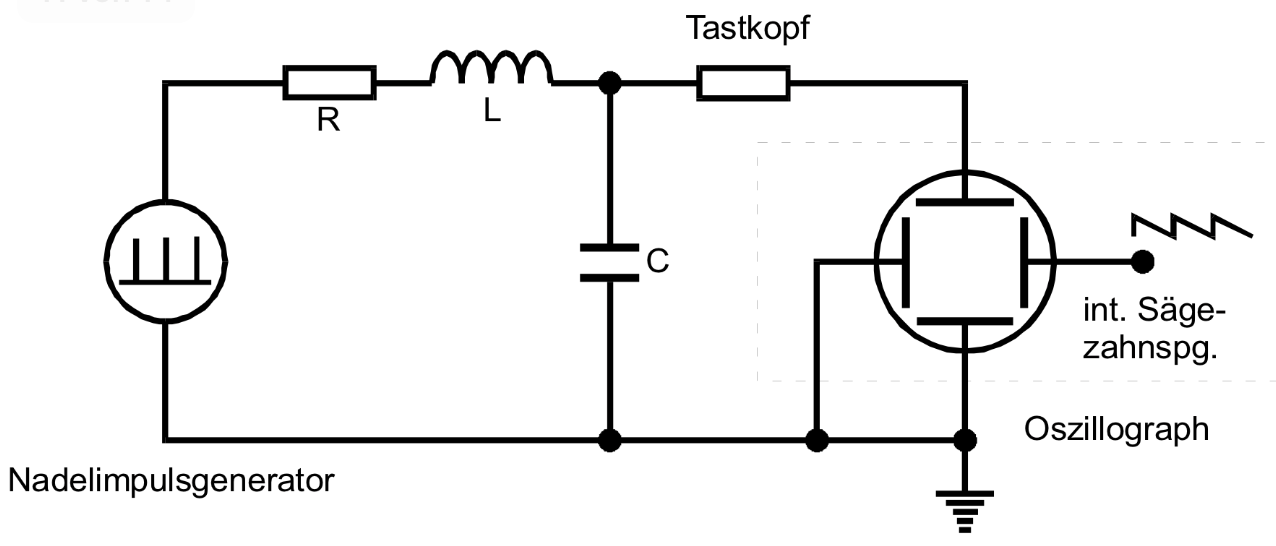
\includegraphics[width=\textwidth]{abb5.jpg}
  \caption{Schaltung zur Untersuchung der Kondensatorspannung\cite{manualV354}}
  \label{fig:abb5}
\end{figure}
Der Nadelpulsgenerator regt den RLC-Schwingkreis zu gedämpften Schwingungen an.
Dabei sollte darauf geachtet werden, dass die Frequenz so gewählt wird, dass vor jedem neuen Impuls $U_C$ um ungefähr den Faktor 3 bis 8 abnimmt.
Für die Messung wird der kleinere der eingebauten Festwiderstände benutzt.
Mit Hilfe des Cursor des digitalen Oszilloskopes können $t$ und $U_C(t)$ der Maxima, die die Einhüllende der Schwingung bilden, abgelesen werden.
Über eine Ausgleichsrechnung werden die gesuchten Größen bestimmt.

\subsection{Dämpfungswiderstand des aperiodischen Grenzfalls}
\label{sec:AufgabeB}

Die Schaltung für diese Messung unterscheidet sich zu Abbildung \ref{fig:abb5} nur durch einen anderen Widerstand.
Dieser kann manuell reguliert werden und wird zu Beginn auf den Maximalwert gestellt.
Anschließend wird der Widerstand $R$ reduziert bis auf dem Oszilloskop der aperiodische Grenzfall zu sehen ist.
Jetzt kann der Dämpfungswiderstand des aperiodischen Grenzfalls $R_{ap}$ an der Schaltung abgelesen werden.

\subsection{Frequenzabhängigkeit der Kondensatorspannung}
\label{sec:AufgabeC}

Die Frequenzabhängigkeit der Kondensatorspannung wird mit einem Schaltkreis wie in Abbildung \ref{fig:abb6} untersucht.
\begin{figure}
  \centering
  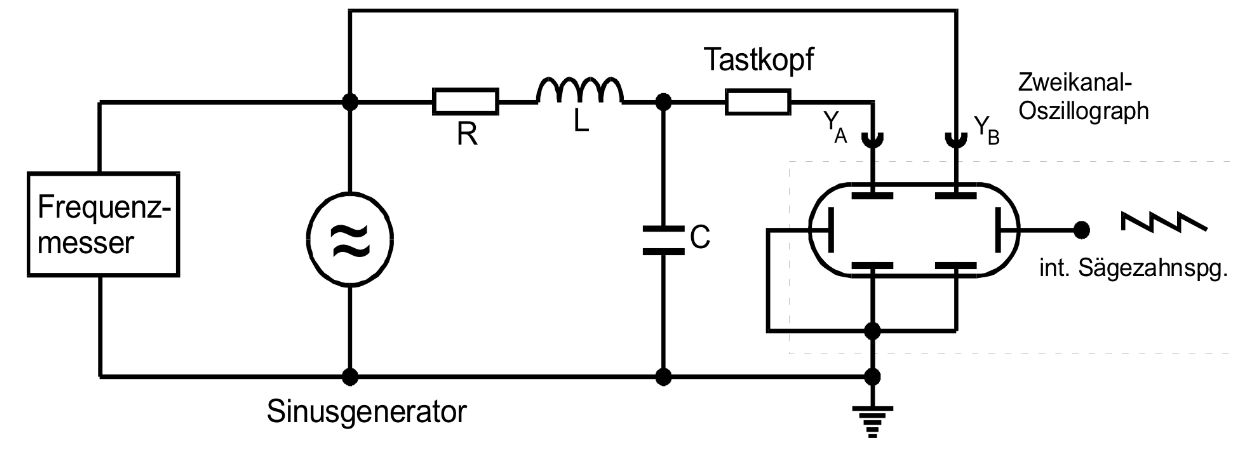
\includegraphics[width=\textwidth]{abb6.jpg}
  \caption{Schaltung zur Untersuchung der Frequenzabhängigkeit von Kondensatorspannung und Phase\cite{manualV354}}
  \label{fig:abb6}
\end{figure}
Gemessen wird mit dem größeren Festwiderstand und die Spannung des Sinusgenerators muss nur einmal zu Beginn bestimmt werden.
Über den Generator werden verschiedene Frequenzen eingestellt und wieder mit Hilfe des Cursors die dazugehörigen Spannungen abgelesen.
In der Nähe der Resonanzfrequenz werden die Messabstände reduziert. Es werden 20 Datenpaare notiert.

\subsection{Frequenzabhängigkeit der Phase von Erreger- und Kondensatorspannung}
\label{sec:AufgabeD}

Die letzte Messung benutzt den gleichen Aufbau wie zuvor und wird auch für die gleichen Frequenzen durchgeführt.
Auf dem Oszilloskop werden die entsprechenden Erreger- und Kondensatorspannungen dargestellt.
Über die Cursorfunktion lässt sich der Abstand der Maxima $a$ ablesen und über die eingestellte Frequenz kann die Periodenlänge $b$ bestimmt werden.
Aus diesen Größen kann dann die Phasenverschiebung berechnet werden.
